\chapter{Radikal, Karbena, dan Penataan Ulang}\label{ch:b3:radicals-carbenes}

Bunga piretrum mempertahankan diri dengan ester-ester asam krisantemat, yaitu molekul
yang dibangun di sekitar cincin karbon beranggota tiga; kerabat-kerabat sintetisnya termasuk
insektisida rumah tangga yang paling banyak dipakai. Para kimiawan menutup cincin semacam itu dalam satu tahap
dengan menambahkan sebuah \omterm{def:b3:organometallic-bonding:carbene}{karbena} pada ikatan rangkap: atom karbon yang hanya dikelilingi enam elektron,
dua di antaranya tidak dipakai bersama. Bab ini membahas zat antara reaktif
yang hanya sepintas dijumpai dalam Jilid Tahun 1 dan Jilid Tahun 2 (radikal yang dipakai dalam
sintesis, \omterm{def:b3:organometallic-bonding:carbene}{karbena}, dan \omterm{def:b3:radicals-carbenes:nitrene}{nitrena}) serta penataan ulang yang memindahkan sebuah gugus
ke atom karbon, nitrogen, atau oksigen yang kekurangan elektron, termasuk dua penataan ulang
yang membuat monomer nilon-6 dan monomer sebuah poliester terbiodegradasi dari
keton yang sama.

\begin{recall}
Jilid Tahun 1 memperkenalkan radikal, homolisis, dan panah berkepala setengah,
karbokation beserta penataan ulangnya, nukleofil, dan gugus pergi; Jilid
Tahun 2 memperkenalkan rantai radikal (inisiasi, propagasi, terminasi, dan inisiator
radikal), asam peroksi, lakton, laktam, dan imina.
\Cref{ch:b3:complex-kinetics} membahas kinetika rantai,
\cref{ch:b3:organometallic-bonding} \omterm{def:b3:organometallic-bonding:carbene}{karbena} sebagai ligan,
\cref{ch:b3:many-electron-atoms} \omterm{def:b3:many-electron-atoms:singlet-triplet}{keadaan singlet} dan triplet, dan
\cref{ch:b3:rate-theories} postulat Hammond.
\end{recall}

\begin{omfigure}
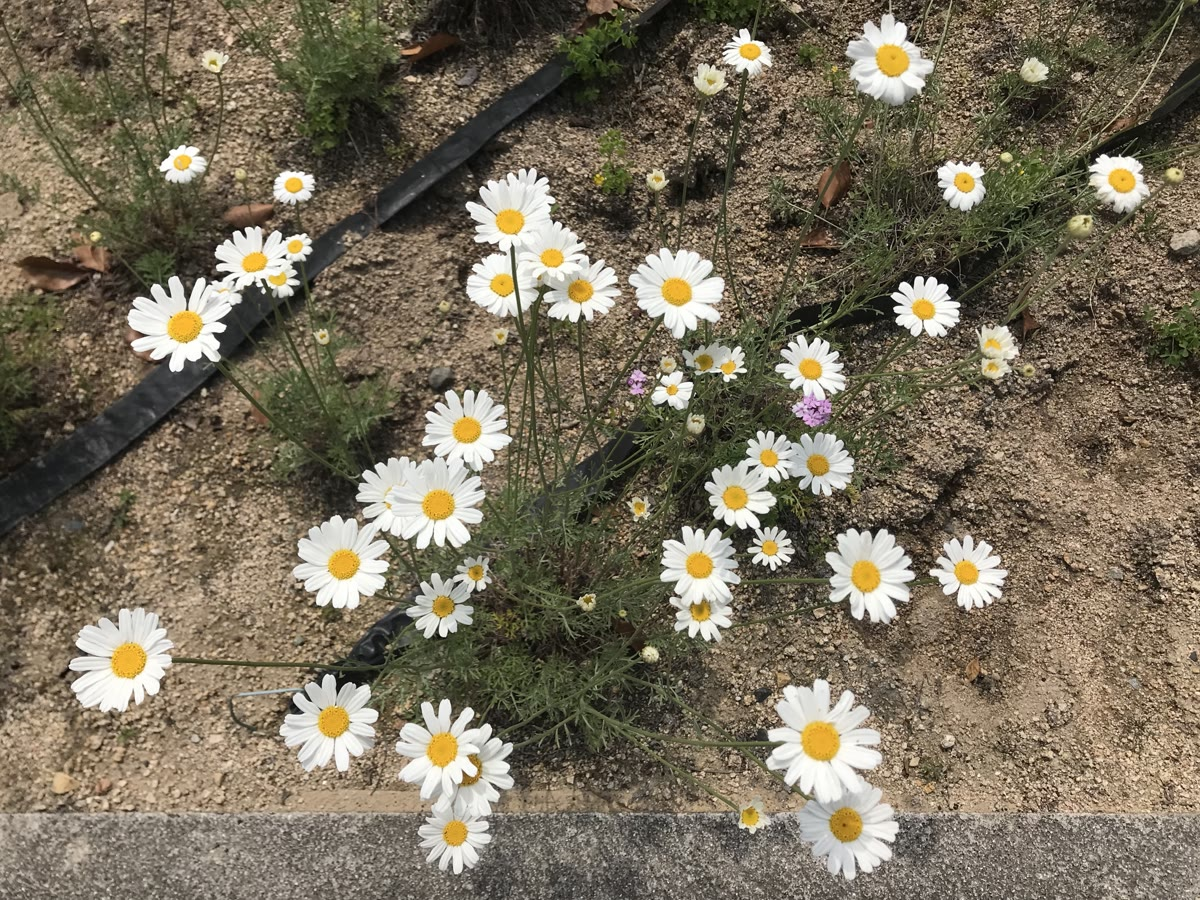
\includegraphics[width=0.48\linewidth]{images/book4/pyrethrum.jpg}

{\small Bunga piretrum. Bunganya mengandung piretrin, yaitu ester insektisidal
sebuah asam siklopropanakarboksilat. Foto: Soramimi, CC BY-SA 4.0.}
\end{omfigure}

\section{Reaksi berantai radikal dalam sintesis}

Kestabilan sebuah radikal karbon diukur dengan entalpi disosiasi ikatan
C--H yang akan membentuknya: makin lemah ikatannya, makin
stabil radikalnya.

\begin{proposition}[Entalpi disosiasi ikatan]\label{prop:b3:radicals-carbenes:bde}
Entalpi disosiasi ikatan R--H pada \qty{298}{K} diperoleh dari entalpi pembentukan
fase gas: $\mathrm{BDE(R{-}H)} = \Delta_fH^\circ(\mathrm R^\bullet) + \Delta_fH^\circ(\mathrm H^\bullet) - \Delta_fH^\circ(\mathrm{RH})$.
\end{proposition}

\begin{proof}
Homolisis $\mathrm{RH \to R^\bullet + H^\bullet}$ memiliki, menurut hukum Hess, entalpi reaksi berupa entalpi
pembentukan produk dikurangi entalpi pembentukan pereaksi; entalpi reaksi itu menurut definisi adalah
entalpi disosiasi ikatan.
\end{proof}

\begin{omfigure}
% ledger: dfh4:CH3r, dfh4:C2H5r, dfh4:iC3H7r, dfh4:tC4H9r, dfh4:PhCH2r, dfh4:H, dfh:CH4_g, dfh:C2H6_g, dfh:C3H8_g, dfh4:iC4H10, dfh4:toluene_g
\begin{tikzpicture}
\begin{axis}[width=0.72\linewidth, height=5.2cm, ybar, bar width=16pt, ymin=350, ymax=450,
  xtick={1,2,3,4,5}, xticklabels={{$\ce{CH3-H}$}, {$\ce{C2H5-H}$}, {$\mathrm{(CH_3)_2CH{-}H}$}, {$\mathrm{(CH_3)_3C{-}H}$}, {$\ce{C6H5CH2-H}$}},
  x tick label style={font=\scriptsize}, ylabel={BDE / \unit{kJ.mol^{-1}}},
  axis lines=left, tick label style={font=\scriptsize}, label style={font=\small},
  nodes near coords, nodes near coords style={font=\scriptsize, /pgf/number format/fixed, /pgf/number format/precision=0},
  enlarge x limits=0.15]
\addplot[fill=omDef!55, draw=omDef] table[x=i, y=bde] {figdata/out/bachelor-3-bde.dat};
\end{axis}
\end{tikzpicture}

{\small Entalpi disosiasi ikatan C--H pada \qty{298}{K}, yang dihitung dari entalpi pembentukan
fase gas molekul-molekul dan radikal-radikalnya: metil, primer,
sekunder, tersier, dan benzilik. Ikatan itu makin lemah ketika radikal yang terbentuk
makin tersubstitusi atau terkonjugasi.}
\end{omfigure}

\begin{proposition}[Selektivitas halogenasi]\label{prop:b3:radicals-carbenes:halogenation-selectivity}
Pengambilan hidrogen oleh atom brom jauh lebih selektif di antara ikatan C--H primer,
sekunder, dan tersier daripada pengambilan oleh atom klor.
\end{proposition}

\begin{proof}[Argumen]
Dengan $\mathrm{BDE(H{-}Cl)}$ lebih besar daripada semua nilai C--H pada gambar dan $\mathrm{BDE(H{-}Br)}$ lebih kecil,
pengambilan oleh klor bersifat eksotermik, sedangkan oleh brom endotermik. Menurut postulat
Hammond (\cref{ch:b3:rate-theories}), keadaan transisi klor terletak awal,
mirip pereaksi, dan hanya sedikit merasakan perbedaan antara radikal-radikal yang terbentuk;
keadaan transisi brom terletak akhir, mirip produk, dan energi aktivasinya mengikuti sebagian besar
perbedaan BDE, yang oleh faktor Boltzmann diubah menjadi rasio laju yang besar.
\end{proof}

Tributiltimah hidrida mereduksi alkil halida melalui sebuah rantai: radikal timah mengambil
halogen, radikal alkil mengambil sebuah atom hidrogen dari molekul hidrida
berikutnya, dan radikal timah yang baru terbentuk. Rantai yang sama menyingkirkan gugus hidroksi
setelah gugus itu diubah menjadi ester tiokarbonil (deoksigenasi Barton--McCombie),
dan menutup cincin. Residu organotimah beracun dan sulit
disingkirkan; tris(trimetilsilil)silana dan silana lainnya kini sering menggantikan timah
hidrida.

\begin{omfigure}
\begin{tikzpicture}[font=\small, >=Stealth]
  \node (a) at (-2.0,0) {$\mathrm{Bu_3Sn^\bullet}$};
  \node (b) at (2.0,0) {$\mathrm{R^\bullet}$};
  \draw[->, thick] (a) to[bend left=35] node[midway, above, font=\scriptsize] {$+\,$R--Br, $\ -\,\mathrm{Bu_3SnBr}$} (b);
  \draw[->, thick] (b) to[bend left=35] node[midway, below, font=\scriptsize] {$+\,\mathrm{Bu_3SnH}$, $\ -\,$R--H} (a);
  \node[font=\scriptsize, align=center, anchor=north] at (0,-1.5) {inisiasi: AIBN $\xrightarrow{\Delta}$ 2 R$'^\bullet$ $+$ $\ce{N2}$; \ R$'^\bullet$ $+$ $\mathrm{Bu_3SnH}$ $\to$ R$'$H $+$ $\mathrm{Bu_3Sn^\bullet}$};
\end{tikzpicture}

{\small Tahap-tahap propagasi reduksi alkil bromida dengan timah hidrida.
Setiap R--Br yang direduksi memakai satu $\mathrm{Bu_3SnH}$ dan memberikan satu $\mathrm{Bu_3SnBr}$; \omterm{def:b3:complex-kinetics:chain}{pembawa
rantainya} adalah radikal timah dan radikal alkil.}
\end{omfigure}

Hidrogen bromida teradisi pada alkena melalui rantai sejenis jika ada
peroksida: atom brom teradisi pada ujung yang kurang tersubstitusi, sehingga terbentuk radikal yang lebih
stabil, yang lalu mengambil atom hidrogen dari HBr: adisi
anti-Markovnikov.

\section{Siklisasi radikal}

\begin{definition}[Siklisasi ekso dan endo]\label{def:b3:radicals-carbenes:cyclisation}
Pada \emph{siklisasi ekso}\index{siklisasi ekso}, ikatan yang putus (atau
ikatan $\pi$ yang diserang) berakhir di luar cincin yang baru; pada \emph{siklisasi
endo}\index{siklisasi endo}, di dalamnya.
\end{definition}

\begin{omfigure}
\begin{tikzpicture}[font=\scriptsize, >=Stealth]
  % radikal heks-5-enil: radikal C1, C5=C6
  \foreach \i/\a in {1/162, 2/234, 3/306, 4/18} { \coordinate (p\i) at (\a:0.9); }
  \coordinate (p5) at (90:0.95); \coordinate (p6) at (90:1.9);
  \draw[thick] (p1) -- (p2) -- (p3) -- (p4) -- (p5);
  \draw[thick, double, double distance=1.5pt] (p5) -- (p6);
  \node[anchor=east] at (p1) {$\bullet$\,1};
  \node[anchor=west] at (p5) {5}; \node[anchor=west] at (p6) {6};
  \draw[->, omMeth, thick] ($(p1)+(0.1,0.15)$) to[bend left=25] node[pos=0.45, below right, inner sep=1pt] {5-ekso} ($(p5)+(-0.15,-0.05)$);
  \draw[->, omThm, thick, densely dashed] ($(p1)+(0,0.25)$) to[bend left=50] node[midway, left] {6-endo} ($(p6)+(-0.2,0)$);
  \node[font=\small, align=center] at (0,-1.6) {radikal heks-5-enil};
  \draw[->, thick] (1.6,0.3) -- (2.7,0.3) node[midway, above] {cepat};
  \begin{scope}[xshift=4.0cm]
    \foreach \i/\a in {1/162, 2/234, 3/306, 4/18, 5/90} { \coordinate (q\i) at (\a:0.75); }
    \draw[thick] (q1) -- (q2) -- (q3) -- (q4) -- (q5) -- (q1);
    \draw[thick] (q5) -- ++(90:0.6) coordinate (q6);
    \node[anchor=south, inner sep=1pt] at (q6) {$\mathrm{{}^\bullet CH_2}$};
    \node[font=\small, align=center] at (0,-1.6) {radikal siklopentilmetil};
  \end{scope}
\end{tikzpicture}

{\small Radikal 5-heksenil menutup melalui serangan C1 pada C5 (5-ekso, hijau): cincin
baru beranggota lima dan radikalnya berakhir di luar cincin, pada C6. Serangan pada C6
(6-endo, putus-putus merah) akan memberikan radikal sikloheksil sekunder yang lebih stabil
tetapi jauh lebih lambat: rantai itu tidak dapat menempatkan C1 pada garis pendekatan ke C6 yang
dituntut orbital $\pi^*$.}
\end{omfigure}

\begin{proposition}[Aturan Baldwin]\label{prop:b3:radicals-carbenes:baldwin}
Untuk penutupan cincin (ditetapkan secara eksperimen, dengan penjelasan
stereoelektronik): pada karbon tetrahedral (tet), 3- sampai 7-ekso disukai, 5- dan
6-endo tidak disukai; pada karbon trigonal (trig), 3- sampai 7-ekso disukai, 3- sampai 5-endo
tidak disukai, 6- dan 7-endo disukai; pada karbon digonal (dig), 3- dan 4-ekso
tidak disukai, 5- sampai 7-ekso disukai, 3- sampai 7-endo disukai.
\end{proposition}

Penjelasannya adalah sudut serangan yang diperlukan setiap jenis ikatan: dari belakang
ikatan pada karbon tet, pada sekitar 107° terhadap sistem $\pi$ trigonal, dan pada sudut yang lebih
sempit terhadap ikatan rangkap tiga; rantai yang pendek tidak dapat menjangkau posisi-posisi itu pada
kasus-kasus yang tidak disukai.

\begin{definition}[Jam radikal]\label{def:b3:radicals-carbenes:radical-clock}
Yang disebut \emph{jam radikal}\index{jam radikal} adalah radikal yang menata ulang
secara unimolekular dengan tetapan laju yang diketahui, seperti radikal 5-heksenil yang
bersiklisasi; persaingannya dengan penangkap bimolekular mengukur tetapan laju
penangkap itu, atau sebaliknya.
\end{definition}

\begin{proposition}[Kinetika kompetisi]\label{prop:b3:radicals-carbenes:clock}
Jika sebuah radikal bersiklisasi ($k_c$) atau ditangkap oleh hidrida yang dijaga berlebih pada
konsentrasi $[\mathrm{R_3SnH}]$ ($k_H$), rasio produknya adalah
$[\text{tersiklisasi}]/[\text{langsung}] = k_c/(k_H[\mathrm{R_3SnH}])$.
\end{proposition}

\begin{proof}
Pada setiap saat, kedua produk terbentuk dengan laju $k_c[\mathrm R^\bullet]$ dan $k_H[\mathrm{R_3SnH}][\mathrm R^\bullet]$. Rasio keduanya
tidak bergantung pada konsentrasi radikal, yang berubah-ubah; dengan konsentrasi hidrida
yang tetap, integrasi terhadap waktu mengalikan keduanya dengan
$\int[\mathrm R^\bullet]\,\dd t$ yang sama, dan rasio produknya adalah rasio tetapan laju
kali $1/[\mathrm{R_3SnH}]$.
\end{proof}

\begin{omfigure}
\begin{tikzpicture}
\begin{axis}[name=a, width=0.47\linewidth, height=5.2cm, xmode=log, xmin=1e-3, xmax=1, ymin=0, ymax=1,
  axis lines=left, xlabel={$[\mathrm{Bu_3SnH}]$ / \unit{mol.L^{-1}}}, ylabel={fraksi tersiklisasi},
  tick label style={font=\scriptsize}, label style={font=\small}]
\addplot[omDef, thick] table[x=c, y=fcyc] {figdata/out/bachelor-3-radical-clock.dat};
\end{axis}
\begin{axis}[at={(a.east)}, anchor=west, xshift=1.5cm, width=0.47\linewidth, height=5.2cm,
  xmin=0, xmax=1, ymin=0, ymax=11, axis lines=left,
  xlabel={$[\mathrm{Bu_3SnH}]$ / \unit{mol.L^{-1}}}, ylabel={[langsung]/[tersiklisasi]},
  tick label style={font=\scriptsize}, label style={font=\small}]
\addplot[omThm, thick] table[x=c, y=inv] {figdata/out/bachelor-3-radical-clock-b.dat};
\node[font=\scriptsize, anchor=west, omThm] at (axis cs:0.15,7.5) {kemiringan $k_H/k_c$};
\end{axis}
\end{tikzpicture}

{\small Jam 5-heksenil dengan tetapan laju model $k_c = \qty{2.3e5}{s^{-1}}$ dan
$k_H = \qty{2.4e6}{L.mol^{-1}.s^{-1}}$. Kiri: fraksi metilsiklopentana di antara produk terhadap
konsentrasi hidrida: setengah pada $k_c/k_H \approx \qty{0.1}{mol/L}$. Kanan: rasio kebalikannya berupa garis
lurus melalui titik asal, dengan kemiringan $k_H/k_c$.}
\end{omfigure}

\begin{method}[Merancang reduksi atau siklisasi radikal]\label{met:b3:radicals-carbenes:radical-chain}
\begin{enumerate}
  \item Untuk reduksi sederhana, jagalah donor hidrogen tetap pekat (sekitar
        \qty{0.1}{mol/L} atau lebih) agar radikalnya tertangkap sebelum menata ulang.
  \item Untuk siklisasi, jagalah donor tetap encer, atau tambahkan perlahan-lahan, agar
        radikal bersiklisasi lebih dahulu: pilihlah $[\text{donor}] \ll k_c/k_H$.
  \item Pilihlah inisiator yang waktu paruhnya pada suhu reaksi berorde
        waktu reaksi (AIBN di dekat \qty{80}{\celsius}), dan tambahkan sedikit demi sedikit jika
        perlu.
  \item Utamakan silana atau donor lain yang bebas timah, dan singkirkan oksigen, yang menangkap
        radikal karbon.
\end{enumerate}
\end{method}

\begin{inthelab}[Penambahan lambat dengan pompa suntik]
Agar sebuah pereaksi tetap encer sepanjang reaksi, larutannya dimasukkan ke dalam
suntikan kedap gas dan ditambahkan melalui septum dengan pompa suntik selama beberapa
jam, ke dalam larutan substrat yang direfluks di bawah nitrogen. Konsentrasi
pereaksi itu lalu tetap di dekat nilai tunaknya yang rendah, yang ditentukan oleh
laju penambahan dan laju pemakaiannya.
\end{inthelab}

\section{Karbena}

\begin{definition}[Karbena singlet dan triplet]\label{def:b3:radicals-carbenes:carbene-states}
Yang disebut \emph{karbena singlet}\index{karbena singlet} adalah \omterm{def:b3:organometallic-bonding:carbene}{karbena} yang kedua elektron nonikatannya
berpasangan dalam satu orbital, yaitu hibrida $sp^2$, dengan orbital p-nya kosong; sedangkan
\emph{karbena triplet}\index{karbena triplet} memiliki kedua elektron itu tidak berpasangan, masing-masing satu di setiap
orbital, dengan spin sejajar.
\end{definition}

\begin{omfigure}
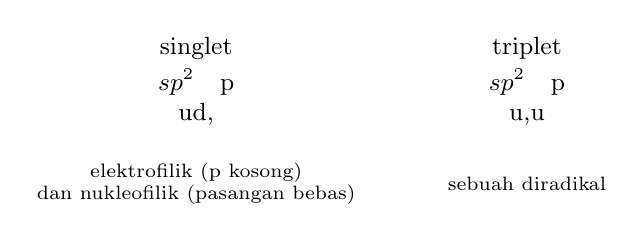
\begin{tikzpicture}[font=\small]
  \node[align=center] at (0,0) {singlet\\[2pt] $sp^2$ \ \ p\\ \omorbs{ud,}};
  \node[align=center] at (4.2,0) {triplet\\[2pt] $sp^2$ \ \ p\\ \omorbs{u,u}};
  \node[font=\scriptsize, align=center] at (0,-1.3) {elektrofilik (p kosong)\\ dan nukleofilik (pasangan bebas)};
  \node[font=\scriptsize, align=center] at (4.2,-1.3) {sebuah diradikal};
\end{tikzpicture}

{\small Okupansi elektron kedua orbital nonikatan sebuah \omterm{def:b3:organometallic-bonding:carbene}{karbena}. Triplet adalah
keadaan dasar $\ce{CH2}$; substituen donor $\pi$ (Cl, gugus OR, $\mathrm{NR_2}$) menaikkan
orbital p dan menjadikan singlet sebagai keadaan dasar, seperti pada diklorokarbena.}
\end{omfigure}

\omterm{def:b3:organometallic-bonding:carbene}{Karbena} dibuat dengan melepaskan dinitrogen dari senyawa diazo (dengan panas, cahaya,
atau katalis logam), melalui eliminasi-$\alpha$ (kloroform dan basa kuat memberikan
$\ce{CCl3-}$, yang melepaskan klorida menjadi $\ce{CCl2}$), atau dihindari sama sekali dengan
sebuah \omterm{def:b3:radicals-carbenes:carbenoid}{karbenoid}.

\begin{definition}[Karbenoid]\label{def:b3:radicals-carbenes:carbenoid}
Yang disebut \emph{karbenoid}\index{karbenoid} adalah spesies yang terikat pada logam yang memindahkan
gugus \omterm{def:b3:organometallic-bonding:carbene}{karbena} seperti \omterm{def:b3:organometallic-bonding:carbene}{karbena} bebas, tanpa terbentuknya \omterm{def:b3:organometallic-bonding:carbene}{karbena} bebas itu,
seperti iodometilzink iodida $\ce{ICH2ZnI}$ pada reaksi Simmons--Smith.
\end{definition}

\begin{definition}[Siklopropanasi]\label{def:b3:radicals-carbenes:cyclopropanation}
Yang disebut \emph{siklopropanasi}\index{siklopropanasi} adalah pembentukan
siklopropana melalui adisi \omterm{def:b3:organometallic-bonding:carbene}{karbena} atau \omterm{def:b3:radicals-carbenes:carbenoid}{karbenoid} pada ikatan rangkap C=C.
\end{definition}

\begin{proposition}[Uji Skell]\label{prop:b3:radicals-carbenes:skell}
\omterm{def:b3:radicals-carbenes:carbene-states}{Karbena singlet} teradisi pada alkena \textit{cis} atau \textit{trans} secara stereospesifik, dengan mempertahankan
konfigurasi relatifnya; \omterm{def:b3:radicals-carbenes:carbene-states}{karbena triplet} memberikan kedua stereoisomer
siklopropana.
\end{proposition}

\begin{proof}[Argumen]
\omterm{def:b3:radicals-carbenes:carbene-states}{Karbena singlet} membuat kedua ikatan baru dalam satu tahap serempak, tanpa waktu untuk
rotasi. \omterm{def:b3:radicals-carbenes:carbene-states}{Karbena triplet} membuat satu ikatan lebih dahulu, sehingga terbentuk 1,3-diradikal triplet; kedua
elektronnya yang tidak berpasangan tidak dapat membentuk ikatan kedua sampai sebuah spin terbalik, dan hal itu
lambat dibandingkan dengan rotasi terhadap ikatan tunggal C--C yang tersisa:
konfigurasinya teracak.
\end{proof}

\begin{omfigure}
\setchemfig{atom sep=1.8em}
\schemestart
\chemfig{H_3C-[:30]=[:0]-[:-30]CH_3}
\arrow{->[$\ce{CH2}$ singlet]}[,1.6]
\chemfig{(<[:210]H_3C)-[:0](<[:330]CH_3)-[:120]-[:240]}
\schemestop
\par\medskip

{\small Uji Skell: \textit{cis}-but-2-ena, dengan kedua gugus metil pada sisi yang sama, memberikan dengan
\omterm{def:b3:radicals-carbenes:carbene-states}{karbena singlet} hanya \textit{cis}-1,2-dimetilsiklopropana (kedua gugus metil pada baji,
pada muka cincin yang sama); dengan \omterm{def:b3:radicals-carbenes:carbene-states}{karbena
triplet}, isomer \textit{trans} juga muncul.}
\end{omfigure}

\omterm{def:b3:radicals-carbenes:carbene-states}{Karbena singlet} juga menyisip ke dalam ikatan C--H. Karboksilat rodium(II)
menguraikan ester diazo menjadi \omterm{def:b3:radicals-carbenes:carbenoid}{karbenoid} rodium yang menyiklopropanasi alkena dan
menyisip ke dalam ikatan C--H secara selektif, dan, dengan ligan kiral, secara enantioselektif.

\begin{definition}[Nitrena]\label{def:b3:radicals-carbenes:nitrene}
Yang disebut \emph{nitrena}\index{nitrena} $\mathrm{R{-}\ddot N}$ adalah analog nitrogen \omterm{def:b3:organometallic-bonding:carbene}{karbena}, yaitu atom
nitrogen netral yang hanya memiliki enam elektron, yang terbentuk misalnya dengan lepasnya
dinitrogen dari sebuah azida.
\end{definition}

\section{Penataan ulang menuju karbon yang kekurangan elektron}

\begin{definition}[Pergeseran-1,2]\label{def:b3:radicals-carbenes:shift}
Yang disebut \emph{pergeseran-1,2}\index{pergeseran-1,2} adalah migrasi sebuah gugus, beserta pasangan
elektron ikatannya, dari satu atom ke atom tetangga yang kekurangan elektron.
\end{definition}

Dalam pergeseran Wagner--Meerwein, gugus alkil atau hidrida berpindah ke karbokation
tetangga, sehingga terbentuk karbokation yang lebih stabil: penataan ulang karbokation pada
Jilid Tahun 1, yang kini diberi nama mekanismenya. Kerangka terpena dibentuk ulang
di alam oleh rangkaian pergeseran semacam itu.

\begin{definition}[Penataan ulang pinakol]\label{def:b3:radicals-carbenes:pinacol}
Yang disebut \emph{penataan ulang pinakol}\index{penataan ulang pinakol} adalah reaksi yang mengubah 1,2-diol,
dalam asam, menjadi keton atau aldehida: satu gugus hidroksi lepas sebagai air, sebuah
gugus pada karbon tetangga bergeser ke kation itu, dan kation yang terbentuk,
yang distabilkan oleh oksigen yang tersisa, melepaskan sebuah proton.
\end{definition}

\begin{definition}[Kecenderungan migrasi]\label{def:b3:radicals-carbenes:migratory}
Yang disebut \emph{kecenderungan migrasi}\index{kecenderungan migrasi} sebuah gugus adalah
kecenderungan relatifnya untuk berpindah dalam \omterm{def:b3:radicals-carbenes:shift}{pergeseran-1,2} ke pusat yang kekurangan elektron.
\end{definition}

Gugus yang membawa muatan positif dengan baik selama pergeseran bermigrasi paling baik: hidrida,
aril, dan alkil tersier lebih dahulu daripada alkil sekunder, primer, dan metil. Pinakol,
$\mathrm{(CH_3)_2C(OH){-}C(OH)(CH_3)_2}$, memberikan pinakolon, 3,3-dimetilbutan-2-on.

\begin{method}[Meramalkan produk penataan ulang]\label{met:b3:radicals-carbenes:rearrangement}
\begin{enumerate}
  \item Carilah atom kekurangan elektron yang terbentuk (kation, nitrenium, oksigen
        peroksida teraktivasi, \omterm{def:b3:organometallic-bonding:carbene}{karbena}, atau \omterm{def:b3:radicals-carbenes:nitrene}{nitrena}) dan gugus pergi yang
        membentuknya.
  \item Daftarlah gugus-gugus pada atom tetangga yang dapat berpindah; jika
        geometrinya tetap (oksim), hanya gugus yang anti terhadap gugus pergi yang dapat berpindah.
  \item Jika tidak demikian, pilihlah berdasarkan \omterm{def:b3:radicals-carbenes:migratory}{kecenderungan migrasi}, atau berdasarkan gugus mana yang membentuk kation
        yang lebih stabil di tempat yang ditinggalkannya.
  \item Pindahkan gugus itu dengan retensi konfigurasinya, lalu lengkapi
        mekanismenya (lepasnya proton, adisi air).
\end{enumerate}
\end{method}

\section{Penataan ulang menuju nitrogen dan oksigen yang kekurangan elektron}

\begin{definition}[Penataan ulang Beckmann]\label{def:b3:radicals-carbenes:beckmann}
Yang disebut \emph{penataan ulang Beckmann}\index{penataan ulang Beckmann} adalah reaksi yang mengubah oksim,
dalam asam kuat, menjadi amida: gugus hidroksi, yang diaktifkan sebagai gugus pergi,
lepas sementara gugus yang anti terhadapnya bermigrasi dari karbon ke nitrogen; air teradisi
pada ion nitrilium yang terbentuk, dan tautomerisasi memberikan amida.
\end{definition}

\begin{proposition}[Migrasi anti]\label{prop:b3:radicals-carbenes:beckmann-anti}
Pada \omterm{def:b3:radicals-carbenes:beckmann}{penataan ulang Beckmann}, gugus yang bermigrasi adalah gugus yang anti terhadap
gugus pergi pada nitrogen.
\end{proposition}

\begin{proof}[Argumen]
Pasangan elektron ikatan yang bermigrasi menyerang nitrogen dari belakang ikatan N--O, seperti pada
substitusi $\mathrm S_\mathrm N2$; hanya gugus yang anti terhadap oksigen yang ikatannya sejajar dengan
orbital $\sigma^*$ N--O. Tahap itu serempak dengan lepasnya gugus pergi,
sehingga tidak terbentuk ion nitrenium bebas yang dapat memilih dengan cara lain.
\end{proof}

\begin{omfigure}
\setchemfig{atom sep=1.9em}
\schemestart
\chemfig{*6(-----(=N-[:30]OH)-)}
\arrow{->[$\ce{H2SO4}$ (oleum)][Beckmann]}[,1.8]
\chemfig{*7(---N(-[:-90]H)-(=O)---)}
\schemestop
\par\medskip
\schemestart
\chemfig{*6(-----(=O)-)}
\arrow{->[asam peroksi][Baeyer--Villiger]}[,1.8]
\chemfig{*7(-----O-(=O)-)}
\schemestop

{\small Dua perluasan cincin sikloheksanon. Atas: oksimnya menata ulang dalam
oleum menjadi kaprolaktam (azepan-2-on), monomer nilon-6, dengan nitrogen memasuki
cincin. Bawah: asam peroksi menyisipkan sebuah atom oksigen di samping gugus
karbonil, sehingga terbentuk $\varepsilon$-kaprolakton (oksepan-2-on).}
\end{omfigure}

\begin{definition}[Oksidasi Baeyer--Villiger]\label{def:b3:radicals-carbenes:baeyer}
Yang disebut \emph{oksidasi Baeyer--Villiger}\index{oksidasi Baeyer--Villiger} adalah reaksi yang mengubah
keton menjadi ester, atau keton siklik menjadi lakton, dengan asam peroksi: asam
peroksi teradisi pada gugus karbonil, lalu sebuah gugus pada karbon karbonil
bermigrasi ke oksigen peroksida yang lebih dekat sementara sebuah karboksilat lepas.
\end{definition}

\begin{proposition}[Regiokimia Baeyer--Villiger]\label{prop:b3:radicals-carbenes:bv-retention}
Pada \omterm{def:b3:radicals-carbenes:baeyer}{oksidasi Baeyer--Villiger}, gugus yang bermigrasi mempertahankan
konfigurasinya, dan urutan \omterm{def:b3:radicals-carbenes:migratory}{kecenderungan migrasinya} adalah alkil tersier >
alkil sekunder $\approx$ aril > alkil primer > metil (urutan yang ditetapkan secara eksperimen).
\end{proposition}

\begin{proof}[Argumen]
Gugus itu berpindah beserta pasangan elektron ikatannya melintasi muka karbon yang ditinggalkannya
dan mendarat pada oksigen dari sisi yang sama, sehingga konfigurasinya dipertahankan. Dalam
keadaan transisi, gugus yang bermigrasi membawa muatan positif parsial, yang
distabilkan oleh substitusi alkil dan konjugasi aril.
\end{proof}

\begin{definition}[Isosianat, penataan ulang Curtius dan Hofmann]\label{def:b3:radicals-carbenes:curtius}
Yang disebut \emph{isosianat}\index{isosianat} adalah senyawa $\ce{R-N=C=O}$. Pada \emph{penataan ulang Curtius}\index{penataan ulang Curtius},
 sebuah asil azida melepaskan dinitrogen jika
dipanaskan sementara gugus R berpindah dari karbon ke nitrogen, sehingga terbentuk isosianat;
pada \emph{penataan ulang Hofmann}\index{penataan ulang Hofmann}, amida primer
yang direaksikan dengan brom dan basa memberikan isosianat yang sama melalui
sebuah N-bromoamida. Dengan air, isosianat memberikan amina $\ce{RNH2}$ dan karbon
dioksida; dengan alkohol, sebuah karbamat.
\end{definition}

\begin{definition}[Keten dan penataan ulang Wolff]\label{def:b3:radicals-carbenes:wolff}
Yang disebut \emph{keten}\index{keten} adalah senyawa $\mathrm{R_2C{=}C{=}O}$. Pada \emph{penataan ulang Wolff}\index{penataan ulang Wolff},
 sebuah $\alpha$-diazoketon melepaskan dinitrogen
sementara gugus pada karbon karbonil bermigrasi, sehingga terbentuk keten, yang mengadisi
air, alkohol, atau amina.
\end{definition}

\omterm{def:b3:radicals-carbenes:wolff}{Penataan ulang Wolff} adalah tahap kunci homologasi Arndt--Eistert,
yang memperpanjang asam karboksilat dengan satu karbon: klorida asam, lalu
diazoketon, lalu \omterm{def:b3:radicals-carbenes:wolff}{keten}, lalu asam homolognya.

\begin{safety}{\ghs[0.62cm]{GHS06}\ghs[0.62cm]{GHS08}\ghs[0.62cm]{GHS09}}
% ledger: ghs4:Bu3SnH, ghs4:diazomethane, ghs4:AIBN
Tributiltimah hidrida: beracun jika tertelan, berbahaya pada kulit, merusak organ pada
paparan berulang, sangat beracun bagi kehidupan akuatik; residu timah dikumpulkan
secara terpisah. Diazometana adalah gas yang beracun, karsinogenik, dan eksplosif; zat itu
disebut di sini hanya karena kimianya dan dalam praktik digantikan oleh pereaksi yang lebih aman
seperti trimetilsilildiazometana. AIBN bersifat swareaktif jika dipanaskan.
\end{safety}

\begin{history}[Radikal yang seharusnya tidak ada, dan sebuah nilon]
Pada 1900 Moses Gomberg, yang mencoba membuat heksafeniletana, memperoleh larutan
kuning yang menyerap oksigen dan iodium: radikal trifenilmetil, radikal karbon
persisten yang pertama. Setengah abad kemudian, \omterm{def:b3:radicals-carbenes:beckmann}{penataan ulang Beckmann}
sikloheksanon oksim menjadi rute industri menuju kaprolaktam, yang dipolimerisasi melalui
pembukaan cincin menjadi nilon-6, sebuah serat dan plastik rekayasa yang dibuat dalam skala
yang sangat besar.
\end{history}

\section{Latihan}

\begin{exercise}[$\star$]\label{exo:b3:radicals-carbenes:1}
Pada \qty{25}{\celsius}, kereaktifan relatif per hidrogen ikatan C--H primer, sekunder, dan
tersier adalah $1 : 3.9 : 5.1$ terhadap atom klor dan $1 : 82 : 1600$ terhadap
atom brom (data latihan). Hitunglah proporsi 1- dan 2-halopropana
yang terbentuk dari propana dalam setiap kasus.
\end{exercise}

\begin{exercise}[$\star$]\label{exo:b3:radicals-carbenes:2}
Manakah keadaan dasar $\ce{CH2}$, dan keadaan dasar $\ce{CCl2}$? Manakah yang teradisi secara stereospesifik pada
\textit{trans}-but-2-ena, dan apa yang dihasilkannya?
\end{exercise}

\begin{exercise}[$\star$]\label{exo:b3:radicals-carbenes:3}
Berikan produk reaksi Simmons--Smith (\textit{Z})-heks-3-ena.
\end{exercise}

\begin{exercise}[$\star$]\label{exo:b3:radicals-carbenes:4}
Berikan produk \omterm{def:b3:radicals-carbenes:baeyer}{oksidasi Baeyer--Villiger} sikloheksanon dan
asetofenon.
\end{exercise}

\begin{exercise}[$\star\star$]\label{exo:b3:radicals-carbenes:5}
Dengan data pada \cref{exo:b3:radicals-carbenes:1}, hitunglah proporsi
kedua monoklorida dan kedua monobromida 2-metilpropana.
\end{exercise}

\begin{exercise}[$\star\star$]\label{exo:b3:radicals-carbenes:6}
Sebuah \omterm{def:b3:radicals-carbenes:radical-clock}{jam radikal} baru, yang direduksi dengan $\qty{0.020}{mol/L}$ $\mathrm{Bu_3SnH}$, memberikan produk tertata ulang tiga kali lebih banyak
daripada produk yang tidak tertata ulang. Dengan $k_H = \qty{2.4e6}{L.mol^{-1}.s^{-1}}$, tentukan tetapan lajunya.
\end{exercise}

\begin{exercise}[$\star\star$]\label{exo:b3:radicals-carbenes:7}
Golongkan menurut aturan Baldwin serangan radikal heks-5-enil pada C5 dan pada C6,
lalu sebutkan apakah setiap penutupan berikut disukai: 4-ekso-tet, 5-endo-trig,
5-ekso-dig, 3-ekso-dig, 5-endo-dig.
\end{exercise}

\begin{exercise}[$\star\star$]\label{exo:b3:radicals-carbenes:8}
Berikan produk \omterm{def:b3:radicals-carbenes:pinacol}{penataan ulang pinakol} 2,3-difenilbutana-2,3-diol,
dan jelaskan pilihan gugus yang bermigrasi.
\end{exercise}

\begin{exercise}[$\star\star$]\label{exo:b3:radicals-carbenes:9}
Benzoil azida dipanaskan dalam toluena, lalu air ditambahkan; dalam percobaan kedua,
etanol. Berikan produk-produknya.
\end{exercise}

\begin{exercise}[$\star\star\star$]\label{exo:b3:radicals-carbenes:10}
Dengan $\mathrm{BDE(H{-}Cl)} = \qty{432}{kJ/mol}$ dan $\mathrm{BDE(H{-}Br)} = \qty{366}{kJ/mol}$ (data latihan) serta nilai-nilai C--H pada
gambar bab ini, hitunglah $\Delta H$ untuk pengambilan hidrogen primer dan hidrogen tersier
oleh setiap atom halogen, dan pakailah postulat Hammond untuk menjelaskan
selektivitas pada \cref{exo:b3:radicals-carbenes:1}.
\end{exercise}

\begin{exercise}[$\star\star\star$]\label{exo:b3:radicals-carbenes:11}
Berikan produk Beckmann kedua oksim, \textit{E} dan \textit{Z}, 2-metilsikloheksanon,
dan jelaskan mengapa keduanya berbeda, sedangkan \omterm{def:b3:radicals-carbenes:baeyer}{oksidasi Baeyer--Villiger} keton itu
memberikan satu lakton utama.
\end{exercise}

\begin{exercise}[$\star\star\star$]\label{exo:b3:radicals-carbenes:12}
Dengan jam model bab ini, hitunglah fraksi tersiklisasi pada $[\mathrm{Bu_3SnH}] = 0.010$,
0.10, dan \qty{1.0}{mol/L}. Konsentrasi hidrida berapakah yang memberikan 95\,\% produk tersiklisasi, dan bagaimana
konsentrasi itu dapat dipertahankan?
\end{exercise}

\section{Soal: Dua Cincin dari Sikloheksanon}

\begin{problem}[{Soal akhir pekan --- dua cincin dari sikloheksanon: oksim,
penataan ulang Beckmann menjadi kaprolaktam, oksidasi Baeyer--Villiger menjadi
kaprolakton, dan regiokimia keduanya dengan 2-metilsikloheksanon}]
\label{pb:b3:radicals-carbenes:1}
% ledger: aw:C, aw:H, aw:N, aw:O, aw:S
Data soal: satu ton sikloheksanon diubah menjadi oksimnya dengan rendemen
98\,\%, dan oksim itu menjadi kaprolaktam dengan rendemen 98\,\%; penataan ulangnya memakai
1.3 mol asam sulfat (sebagai oleum) per mol oksim, yang pada akhirnya dinetralkan dengan
amonia menjadi amonium sulfat.

\medskip\noindent\textbf{Bagian I --- Oksim.}
\begin{enumerate}[beginpenalty=10000]
  \item Tuliskan pembentukan sikloheksanon oksim dari hidroksilamina.
  \item Mengapa reaksi itu dijalankan di dekat pH 4 sampai 5?
  \item Apakah sikloheksanon oksim memiliki isomer \textit{E} dan \textit{Z}? Mengapa?
  \item Gambarlah oksim \textit{E} dan \textit{Z} 2-metilsikloheksanon.
  \item Mengapa kedua oksim ini hanya lambat saling berubah?
\end{enumerate}

\medskip\noindent\textbf{Bagian II --- \omterm{def:b3:radicals-carbenes:beckmann}{Penataan ulang Beckmann}.}
\begin{enumerate}[resume, beginpenalty=10000]
  \item Apakah yang dilakukan asam terhadap oksim?
  \item Ikatan manakah yang bermigrasi, dan mengapa migrasi itu memperbesar cincin?
  \item Zat antara apakah yang diserang air?
  \item Tuliskan persamaan keseluruhannya, dari oksim ke kaprolaktam.
  \item Namailah dan gambarlah produknya, beserta polimer yang dibuat darinya.
  \item Hitunglah massa molar sikloheksanon dan kaprolaktam.
  \item Hitunglah massa kaprolaktam dari satu ton sikloheksanon.
  \item Hitunglah massa amonium sulfat yang ikut terbentuk.
\end{enumerate}

\medskip\noindent\textbf{Bagian III --- \omterm{def:b3:radicals-carbenes:baeyer}{Oksidasi Baeyer--Villiger}.}
\begin{enumerate}[resume, beginpenalty=10000]
  \item Tuliskan oksidasi sikloheksanon oleh asam peroksi $\ce{RCO3H}$.
  \item Berikan zat antara yang terbentuk melalui adisi asam peroksi.
  \item Gugus manakah yang bermigrasi, dan apakah gugus perginya?
  \item Namailah lakton itu dan polimer yang dihasilkannya.
  \item Mengapa hidrogen peroksida dengan katalis dapat menggantikan asam peroksi dalam
        proses yang lebih bersih?
\end{enumerate}

\medskip\noindent\textbf{Bagian IV --- 2-Metilsikloheksanon.}
\begin{enumerate}[resume, beginpenalty=10000]
  \item Karbon manakah yang bermigrasi dalam \omterm{def:b3:radicals-carbenes:baeyer}{oksidasi Baeyer--Villiger-nya}, dan lakton apakah yang terbentuk?
  \item Apakah konfigurasi karbon itu dipertahankan?
  \item Laktam manakah yang diberikan oleh oksim \textit{E} (OH anti terhadap karbon yang membawa metil)?
  \item Laktam manakah yang diberikan oleh oksim \textit{Z}?
  \item Apakah yang menentukan regiokimia dalam setiap reaksi?
  \item Mengapa sikloheksanon sendiri bebas dari masalah-masalah ini?
  \item Nyatakan hasilnya: massa kaprolaktam dari satu ton sikloheksanon.
\end{enumerate}
\end{problem}
